% !TeX spellcheck = en_US
\documentclass[12pt]{report}
\usepackage{paccopsde}
	\makeindex
\begin{document}
	\title{Partial Stochastic Differential Equations}
	\author{Kotatsu}
	\date{\small TOALDO VAFFANCULOOOOOOOOOO}
	\maketitle
	\pagenumbering{Roman}
	\begin{preface}
		These are the notes of the Stochastic Processes course for the Academic Year 2025-2026 with Professors Toaldo and Badiale.\par
		I took these notes personally and I integrated the (many) unclear parts and passages using online resources and occasionally the fucking shitty books that this course has. \par
		\vskip1.2cm
		
		\hfill Kotatsu
		\vskip1.2cm
		Check the source code for this and other notes in my GitHub repo $\to$ \href{https://github.com/godblessourdeadkotatsu/lecture-notes-2024-25/tree/main/PSDE}{\faGithubSquare}
	\end{preface}
	\clearpage
	\tableofcontents
	\pagenumbering{arabic}
\chapter{The Itô integral}	
\section{Introduction}
Imagine we have a random phenomenon whose realization is 
\begin{equation*}
	\seqtm{X}.
\end{equation*}
Imagine the infinitesimal increment 
\begin{equation*}
	\seqtdt{X}.
\end{equation*}
This is proportional to the time integral
\begin{equation*}
	\seqtdt{X}=X_{t}=b\dt
\end{equation*}
which is just a deterministic quantity proportional to the time increment $\dt$. Now add a source of randomness like a noise \rv{} $Z$:
\begin{equation*}
	b\dt+\sigma Z.
\end{equation*}
When we model something random we usually have a deterministic to which we add some noise. We can see $Z$ as the total contribution of $N$ (small) sources of randomness:
\begin{equation*}
	Z=\sum_{i=1}^{N}\frac{X_{i}}{N}.
\end{equation*}
If the $X_{i}$ are i.i.d. then $Z$ is gaussian with $Z\distnorm{0,1}$. We can imagine that $Z$ increases with time (the more time it passes, the more the ``noise'' can influence the process) so we can think of $Z$ as 
\begin{equation*}
	Z\distnorm{0,\dt}.
\end{equation*}
We now have 
\begin{equation*}
	\dif X_{t}=b\dt+\sigma Z
\end{equation*}
which is already a stochastic differential equation (SDE) in the way we usually write it. We can think of $Z$ as the increment of a \bwm{}:
\begin{equation*}
	Z=B_{t+\dt}-B_{t}\implies \dif X_{t}=b\dt+\sigma\dbt.
\end{equation*}
We could imagine that the variation of $X$ and the effect of the noise are dependent on the current position of the process $X_{t}$:
\begin{equation*}
	\dxt=b(X_{t})\dt+\sigma(X_{t})\dbt.
\end{equation*}
In this scenario, to know the future evolution of the process we just have to know the position of the process in the current time: this is indeed the differential equation of a \emph{Markovian process}.
We have to remember that 
\begin{equation*}
	\dxt=b(X_{t})\dt+\sigma(X_{t})\dbt
\end{equation*}
is just a symbol. If this was ``literal'' then it would mean
\begin{equation*}
	\frac{\dif}{\dt}X_{t}=b(X_{t})+\sigma(X_{t})\frac{\dif}{\dt}B_{t}
\end{equation*}
but this \emph{doesn't make any fucking sense} because we know that the \bwm{} is not differentiable in any point. To get around this a common trick is to write the integral equation
\begin{equation*}
	X_{t}-X_{0}=\ubracketthin{\int_{0}^{t}b(X_{s})\ds}_{\claptext{Normal Riemann integral}}+\int_{0}^{t}\sigma(X_{s})\dif B_{s}.
\end{equation*}
The $\int_{0}^{t}\sigma(X_{s})\dif B_{s}$ part could look like a normal Riemann - Stieltjes integral (the ones of the kind $\int_{A}f(x)\dif g(x)$ where we ``weigh'' each piece of a function with another) but the problem is that we cannot use a single trajectory of a \bwm{} for this. \bwm{} has infinite variation and therefore the sums could diverge. The tools we have for analysis are not general enough for the class of functions we are trying to study. To understand the object
\begin{equation*}
	\int_{0}^{t}B_{s}\dbs
\end{equation*}
we need a new notion of integral. Once we know what this is then our SDE is just a normal differential equation system, whose solution turns out to be a process called \emph{Itô diffusion}. We will see that these diffusions help us solve PDSE in general. All \ito{} diffusions can be written as
\begin{equation*}
	\frac{\partial}{\partial t}q(x,t)=G_{x}q(x,t)\qquad q(x,0)=u(x)
\end{equation*}
where $G_{x}$ is a linear operator and where 
\begin{equation*}
	\evs^{x}u(X_{t}) 
\end{equation*}
is the solution. This is a huge class of functions called \textit{parabolic equations} and they allow us to use probabilistic methods also for general analytic equations.
\section{Some facts about \bwm{} construction}
We already know how to construct a trajectory (that is a probability space) that satisfies all the conditions for a \bwm{} trajectory by computing the increments. It is a probability space $(\Omega,\A,\pr)$ of the kind
\begin{equation*}
	\left(\mathcal{C}_{0}(I),\B,P_{\omega}\right)
\end{equation*}
with $I=[0,\infty)$. Which \sa{} can we construct on a function space and which probability measure $P_{\omega}$ is such that the collection
\begin{equation*}
	B(\omega)=\seqttm{B_{t}(\omega)}
\end{equation*}
is a \bwm? There are a lot of ways to construct a \bwm{} but just one can be extended to Markov processes and this is the \emph{canonical construction of a \bwm}. \par
Let $I=[0,\infty)$: for each $t\in I$ let $(E_{t},\E_{t})$ be a measurable space. The collection ${\left(X_{t}\right)}$ can be viewed as a function $I\ni t\mapsto X_{t}\in E_{t}$. In most case we simply have $(E_{t},\E_{t})=(\R,\B(\R))$. The product space 
\begin{equation*}
	F=\bigtimes_{t\in I}E_{t}
\end{equation*}
Is the set of such $X$; that is, the set of all real valued functions from $I$ to $E_{t}$. The correspondent \sa{} is 
\begin{equation*}
	\bigotimes_{t\in I}\Sigma_{t}=\sigma(\text{measurable rectangle}).
\end{equation*}
\begin{definition}
	A rectangle in $F$ is a subset
	\begin{equation*}
		\left\{X\in F:X_{t}\in A_{t}\qquad\every t\in I\right\}
	\end{equation*}
	and this is the subset of functions $A_{t}$ that differs from $E_{t}$ only in a finite number of positions $t\in I$.
\end{definition}
A cylinder set is obtained by restricting finitely many coordinates to measurable subset $A_{t}$
and leaving all other coordinates unrestricted.
\begin{figure}[h]
	\centering
	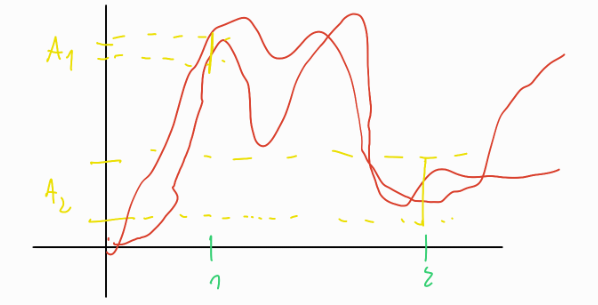
\includegraphics[width=0.7\linewidth]{img/screenshot001}
	\caption{All the functions that are in area 1 at time 1 and in area 2 at time 2 are included in the rectangle}
	\label{fig:screenshot001}
\end{figure}
A random process is a sequence of \rv s but it can also be seen as a one \rv{} measurable on the product space. If $I=[0,\infty)$ then the product space is $\R^{(0,\infty)}$. So we now need to explicitly build a process that is a random process.
\begin{theorem}
	For $t_{1},\ldots,t_{n}\geq0$ with $n\in\N$ and $t_{j}\neq t_{i}$ we assume that 
	\begin{equation*}
		P_{t_{1},\ldots,t_{n}}(\cdot)
	\end{equation*}
	is a family of probability measures for any choice of $n$ and it is on $\left(\R^{n},\B(\R^{n})\right)$.
The Kolmogorov consistency conditions tell us that this family has a random process having this as a distribution. The conditions are:
\begin{enumerate}
	\item $P_{t_{1},\ldots,t_{n}}(A_{1}\times\ldots\times A_{n})=P_{t_{\sigma(1)},\ldots,t_{\sigma(n)}}(A_{\sigma(1)},\ldots,A_{\sigma(n)})$, which means that the distribution is invariant to permutations;
	\item $P_{t_{1},\ldots,t_{n}}(A_{1},\ldots,A_{n-1}\times \R)=P_{t_{1},\ldots,t_{n-1}}(A_{1}\times\ldots\times A_{n-1})$ (integrating the marginal).
\end{enumerate}
If we can specify our family such that $t_{1}<t_{2}<\ldots<t_{n}$ then there exists a unique probability measure $\mu$ on the product space $(\R^{I},\B^{I}(\R))$ such that the canonical process
\begin{equation*}
	X_{t}(\omega)=\omega,\qquad X=\seqtm{X}
\end{equation*}
has finite dimensional distribution $P_{t_{1},\ldots,t_{n}}$. 
\end{theorem}
Now take $t_{1}<t_{1}<\ldots<t_{n}$ and 
\begin{equation*}
	T_{t_{1},\ldots,t_{n}}\distnorm{0,\mathbf{C}}
\end{equation*}
with covariance matrix
\begin{equation*}
	\mathbf{C}_{ij}=t_{i}\wedge t_{j}.
\end{equation*}
This is just the finite dimensional \bwm{} distribution. The idea behind all of this thing is that once we choose the canonical process, finding a probability measure $P$ on $(\Omega,\B^{I}(\R))$ automatically determines the finite-dimensional distribution of this process. Vice versa, if we start from a family of finite-dimensional distribution that satisfy the Kolmogorov extension theorem conditions, then we can define a measure $P$ such that the canonical process has those particular distributions.
\begin{corollary}
	If $\seqtm{X}$ is a process then there exists a unique measure $\mu$ on the product space such that the canonical process satisfies $X_{0}=0$, then $X_{t}$ has stationary independent and Gaussian increments.
\end{corollary}
Product \sa{} is generated by measurable rectangles, typically by union or intersection; but that is just the combination of a countable number of information and we need to understand what to do when the information is uncountable. We care about this because to create a probability measure on our event space we need some kind of \sa{} and the product \sa{} is the \emph{smallest \sa{}} that makes all projection of the canonical process measurable.
\begin{theorem}
	For every $\Gamma\subset \B^{I}(\R)$ there exists an \textit{at most} countable set $S\subset I$ such that 
	\begin{equation*}
		v\in\Gamma,w\in\R^{I}\;\text{and}\;v|_{S}=w|_{S}\implies w\in\Gamma.
	\end{equation*}
\end{theorem}
This tells us that the product \sa{} is too small: for any set in the \sa{} (countably generated) we can find a set of indices which depends on $\Gamma$ and it is countable. If we pick a function  $v$ in $\Gamma$ and we choose another function $w$ in $\B^{I}(\R)$ coinciding with $v$ on $S$ then it must belong to $\Gamma$ as well... but $w$ may be not continuous! This means that the set of continuous functions $C_{0}(I)$ is \underline{not} in $\B^{I}(\R)$. This is an issue because it implies that the set $C_{0}(I)$ is not measurable with respect to the product \sa{} so we cannot compute a probability measure on it.
\begin{equation*}
	\mathcal{C}_{0}([0,\infty))\notin\B^{[0,\infty)}.
\end{equation*}
Define the following metric between functions:
\begin{equation*}
	\rho(v,w):=\sum_{n\geq1}2^{-n}\min\left\{\sup_{0\leq t\leq n}|v(t)-w(t)|,1\right\}
\end{equation*}
so that if $\rho(v_{n},v)\to0$ then $v_{n}\to v$. This also gives us uniformity on a compact set. This metric space is separable, which means that there exists a dense numerable subset in this space. Here $\B(\mathcal{C}_{0}(I))$ is the smallest that contains
\begin{equation*}
	B_{\rho}(\mu,r):=\left\{v\in\mathcal{C}_{0}(I):\rho(\mu,v)< r\right\}
\end{equation*}
which is the open Borel ball.
\begin{lemma}
	We have
	\begin{equation*}
		\B^{I}(\R)\cap \mathcal{C}_{0}(I)=\B(\mathcal{C}_{0}(I)).
	\end{equation*}
\end{lemma}
This means that the Borel \sa{} on $\mathcal{C}_{0}(I)$ induced by $\rho$ is equal to the trace \sa{} obtained by restricting the product \sa{} $\B^{I}(\R)$ to the set $\mathcal{C}_{0}(I)$.
\begin{definition}
	If $(E,\E)$ is a measurable space and $F\subset E$ then the trace \sa{} on $F$ is
	\begin{equation*}
		\Sigma_{F}:=\left\{A\cap F:A\in\E\right\}.
	\end{equation*}
\end{definition}
\begin{theorem}
	Let $X=\seqtm{X}$ be a $d$-dimensional process on $(\Omega,\A,\pr)$. If there are constants $c,\alpha,\beta$ all $>0$ such that
	\begin{equation*}
		\ev{\left|X_{t}-X_{s}\right|^{\alpha}}\leq c|t-s|^{1+\beta}
	\end{equation*}
	then $X_{t}$ has a version with \emph{only continuous paths}.
\end{theorem}
\begin{revise}
	The version of a \rv{} is a \rv{} $\Xbar$ such that
	\begin{equation*}
		\pr(X_{t}=\Xbar_{t})=1\qquad\every t
	\end{equation*}
\end{revise}
In particular, for \bwm{} we have that
\begin{equation*}
	\ev{\left|X_{t}-X_{s}\right|^{4}}=\ev{\left|X_{t-s}\right|^{4}}=\ubracketthin{|t-s|^{2}}_{\sigma^{4}}\ubracketthin{\ev{\left|X_{t}\right|^{4}}}_{3=c}
\end{equation*}
so there exists a version with continuous paths. Let's denote it as
\begin{equation*}
	\Xbar=\seqtm{\Xbar}\qquad\Xbar(\omega)\in\mathcal{C}_{0}(I).
\end{equation*}
Now take a measure $\mu$ and define
\begin{equation*}
	P(A):=\mu\left(\left\{\omega\in\R^{I}:\Xbar(\omega)\in A\right\}\right).
\end{equation*}
This is the image measure of $\mu$ under $\Xbar$:
\begin{equation*}
	P=\mu\circ\Xbar^{-1}.
\end{equation*}
By Kolmogorov extension theorem we get
\begin{equation*}
	\left(\R^{I},\B^{I}(\R),\mu\right)\xrightarrow{\Xbar}\left(\mathcal{C}_{0}(I),\B(C_{0}(I)),P\right)
\end{equation*}
where $P$ is the image measure of $\mu$ called \emph{Wiener measure}. So by construction $\left(\mathcal{C}_{0}(I),\B(C_{0}(I)),P\right)$ is a probability space where the canonical process is \bwm{} with continuous paths.
\section{More facts about \bwm{} trajectories}
Take $f:[0,\infty]\mapsto\R^{d}$. Ideally, $f(t)=B(t,\omega)$. We want to measure the oscillations off the interval $[a,b]$. Set 
\begin{equation*}
	a=t_{0}<t_{1}<\ldots<t_{n}=b
\end{equation*}
and call $[a,b]=\Pi$.
\begin{definition}
	Let $f:[0,\infty)\to\R^{d}$ and let $\seqn{\Pi}$ with $n\in\N$ be a sequence of a partition of $[0,t]$ with mesh $\left|\Pi_{n}\right|\to0$, Then 
	\begin{equation*}
		\vari_{p}(f,t):=\lim_{n\to\infty}S^{\Pi_{n}}_{p}(f,t)
	\end{equation*}
	is called \emph{$p$-variation of $f$ along $\Pi$}.
\end{definition}
 We denote the following quantity
\begin{equation*}
	\sum_{t_{j}\leq\Pi}\left|f(t_{j})-ft_{j-1})\right|^{P}=S^{\Pi}_{p}(f,[a,b])
\end{equation*}
as the \emph{$p$-variation sum} of $f$ on $[a,b]$ along the partition path.
\begin{definition}
	Let $f:[0,\infty)\to\R^{d}$ and $\Pi:=\left\{
	0=t_{0}<t_{1}<\ldots<t_{n}=t\right\}$ with mesh $|\Pi|:=\max_{j}|t_{j}-t_{j-1}|$. for $p>0$ we call
	\begin{align*}
		S_{p}^{\Pi}(f,t)&=\sum_{t_{j}\leq\Pi}\left|f(t_{j})-f(t_{j-1})\right|^{p}\\
		&=\sum_{j=1}^{n}\left|f(t_{j})-f(t_{j-1})\right|^{p}
	\end{align*}
	the \emph{$p$-variation sum of f along $\Pi$} and we call
	\begin{equation*}
		\vari_{p}(f,t)=\sup\left\{S^{\Pi}_{p}(f,t):\Pi\text{ is a partition of }[0,t]\right\}
	\end{equation*}
	the \emph{strong $p$-variation}.
\end{definition}
The difference with the weak $p$-variation is that the strong $p$-variation is for any partition and not just along a sequence. We have that
\begin{equation*}
	S_{2}^{\Pi_{n}}(B,t)\xrightarrow{L^{2}}t
\end{equation*}
and there exists a subsequence $\seqkk{\Pi_{n_{k}}}$ of partitions such that
\begin{equation*}
	S^{\Pi_{n_{k}}}_{2}(B,t)\convas t
\end{equation*}
and there exists a sequence $\seqn{\Pi}$ such that
\begin{equation*}
	S^{\Pi_{n}}:S_{2}^{\Pi_{n}}(B,t)\convas t \qquad\text{if }\sum_{n}|\Pi_{n}|\leq\infty.
\end{equation*}
\begin{proposition}
	For any $t>0$ and $p\leq2$ we have
	\begin{equation*}
		\vari_{p}(B,t)=+\infty.
	\end{equation*}
\end{proposition}
\begin{fancyproof}
	We prove for $p<2$. Choose $p=2-\delta$ for $\delta>0$ and let $\seqn{\Pi}$ be a sequence of partitions such that $|\Pi_{n}|\to0$. Then, if we suppose that $\vari_{p}(B,t)<\infty$, we expect $\sum_{t_{j}\in\Pi_{n}}\left(B_{t_{j}}-B_{t_{j-1}}^{2}\right)\leq\vari_{p}(B,t)<\infty$. We can write
	\begin{align*}
		\sum_{t_{j}\in\Pi_{n}}\left(B_{t_{j}}-B_{t_{j-1}}^{2}\right)&=\sum_{t_{j}\in\Pi_{n}}\left(B_{t_{j}}-B_{t_{j-1}}\right)^{\delta}\left(B_{t_{j}}-B_{t_{j-1}}\right)^{2-\delta}\\
		&\leq\max_{t_{j}\in\Pi_{n}}\left|B_{t_{j}}-B_{t_{j-1}}\right|^{\delta}\sum_{t_{j}\in\Pi_{n}}\left|B_{t_{j}}-B_{t_{j-1}}\right|^{2-\delta}\\
		&\leq\max_{t_{j}\in\Pi_{0}}\ubracketthin{\left|B_{t_{j}}-B_{t_{j-1}}\right|^{\delta}}_{\to0}\vari_{p}(B,t)=0
	\end{align*}
	but this is a contradiction because we know that 
	\begin{equation*}
		\sum_{t_{j}\in\Pi_{n}}\left|B_{t_{j}}-B_{t_{j-1}}\right|\xrightarrow{|\Pi|\to0}=t
	\end{equation*}
	that is, the quadratic variation goes to $t$ and not 0!
\end{fancyproof}
\begin{theorem}
	Let $\seqtm{B}$ be a 1-dimensional \bwm. If $\seqn{\Pi}$ is a sequence of partitions on $[0,t]$ with $\left|\Pi_{n}\right|\to0$ then the quadratic variation is such that $$\vari_{2}(B,t)=L^{2}-\lim_{n}S_{n}^{\Pi_{n}}(B,t).$$
\end{theorem}
\begin{fancyproof}
	We actually mean to prove 
	\begin{equation*}
		\ev{\left(S^{\Pi}_{2}(B,t)-t\right)^{2}}\xrightarrow{|\Pi|\to0}0.
	\end{equation*}
	Set $\Pi=\left\{0=t_{0}<t_{1}<\ldots<t_{n}\right\}$. Since $\ev{S_{2}^{\Pi}(B,t)}=t$, we have
	\begin{align*}
		\ev{\left(S^{\Pi}_{2}(B,t)-t\right)^{2}}&=\ev{\left(S^{\Pi}_{2}(B,t)-\ev{S_{2}^{\Pi}(B,t)}\right)^{2}}\\
		&=\var\left(S_{2}^{\Pi}(B,t)\right).
	\end{align*}
	We have
	\begin{align*}
		\ev{S^{\Pi}_{2}(B,t)}&=\sum_{j=1}^{n}\ev{\left(B_{t_{j}}-B_{t_{j-1}}\right)^{2}}\\
		&=\sum_{j=1}^{n}(t_{j}-t_{j-1})=t.
	\end{align*}
	Moreover,
	\begin{align*}
		\ubracketthin{\var\left(\sum_{j=1}^{n}(B_{t_{j}}-B_{t_{j-1}})^{2}\right)}_{\var\left(S_{2}^{\Pi}(B,t)\right)}&=\sum_{j=1}^{n}\ev{\left((B_{t_{j}}-B_{t_{j-1}})^{2}-(t_{j}-t_{j-1})\right)^{2}}\\
		&\text{by indep. increments}\\
		&=\sum_{j=1}^{n}\ev{\left(B^{2}_{t_{j}-t_{j-1}}-(t_{j}-t_{j-1})\right)^{2}}\\
		&=\sum_{j=1}^{n}(t_{j}-t_{j-1})^{2}\ubracketthin{\ev{\left(B_{t}^{2}-1\right)}}_{c}\\
		&\text{by scaling property}\\
		&=c\sum_{j=1}^{n}\ubracketthin{(t_{j}-t_{j-1})}_{\leq|\Pi|}(t_{j}-t_{j-1})\\
		&\leq c|\Pi|t\xrightarrow{|\Pi|\to0}0
	\end{align*}
\end{fancyproof}
\section{\ito{} integral: definition and properties}
Consider the Riemann integral: if the limit for the partition of the superior and inferior sum exists then we have
\begin{equation*}
	\lim_{|\Pi_{n}|}R^{\Pi_{n}}=\int_{a}^{b}f(s)\ds.
\end{equation*}
Now think about the Riemann-Stieltjes integral
\begin{equation*}
	\int_{b}^{a}f(s)\dif g(s).
\end{equation*}
This comes from the sum
\begin{equation*}
	R^{\Pi_{n}}_{g}=\sum_{j=0}^{n-1}f(\xi_{j})(g(x_{j_1})-g(x_{j}))
\end{equation*}
and then taking the limit
\begin{equation*}
	\lim_{|\Pi_{n}|}R_{g}^{\Pi_{n}}=\int_{a}^{b}f(s)\dif g(s).
\end{equation*}
The conditions for the Riemann-Stieltjes integral to exist are:
\begin{enumerate}
	\item $f$ and $g$ have no joint discontinuities (necessary);
	\item $f$ is continuous, $g$ is of bounded variation (sufficient);
	\item $f$ and $g$ must have no joint discontinuities and $f$ has bounded $p$-variation and $g$ has bounded $q$-variation with
	\begin{equation*}
		\frac{1}{p}+\frac{1}{q}=1.
	\end{equation*}
\end{enumerate}
This last condition is not sufficient but it's very hard to find functions that do not adhere to it. One of these functions is \bwm.
\begin{proposition}
	Let $g:[a,b]\to\R$ and denote
	\begin{equation*}
		I(f):\int_{a}^{b}f(t)\dif g(t)
	\end{equation*}
	in the Riemann-Stjelties sense. If $I(f)$ exists for any $f\in\mathcal{C}([a,b])$ then $g$ is of bounded variation.
\end{proposition}
This is one of the analytical reasons why we actually cannot use RS integrals for \bwm: if such an integral existed, then \bwm{} would have to be of bounded variation and this is not possible.
\begin{fancyproof}
	To prove this we need to use the Banach Steinhaus theorem.
	\begin{theorem}
		\emph{Banach Steinhaus theorem}. Let $\normsp{X}$ and $\normsp{Y}$ be Banach spaces and let $I$ be a set of indices. For each $i\in I$ let $S_{i}:X\to Y$ be a continuous and linear mapping. If
		\begin{equation*}
			\sup_{i\in I}\norm{S_{i}(x)}_{Y}<\infty\qquad x\in X
		\end{equation*}
		then
		\begin{equation*}
			\sup_{i\in I}\sup_{\norm{x}_{X}\leq 1}\norm{S_{i}(x)}_{Y}<\infty.
		\end{equation*}
	\end{theorem}
	We use Banach-Steinhaus with $X=\mathcal{C}([a,b])$ and $Y=\R$ and $I$ as the set of finite positions
	\begin{equation*}
		\Pi=\left\{a=t_{0}<\ldots<t_{n}=b\right\}.
	\end{equation*}
	Define
	\begin{equation*}
		S_{\Pi}(f):=\sum_{i-1}^{n}f(t_{i})(g(t_{i})-g(t_{i-1}))
	\end{equation*}
	as the Riemann-Stieltjes sum
	and note that this is a linear operator. We have
	\begin{align*}
		\left|S_{\Pi}(f)\right|&\leq\norm{f}_{\infty}\sum_{i=1}^{n}\left|g(t_{i})-g(t_{i-1})\right|\\
		&=c_{\Pi,g}\norm{f}\infty.
	\end{align*}
	$S_{\Pi}$ is bounded, so it is continuous. We have that
	\begin{equation*}
		S_{\Pi}(f)\to\int_{a}^{b}f(t)\dif g(t)\qquad\every f\in\mathcal{C}([a,b])
	\end{equation*}
	and when $|\Pi|\to0$ we have
	\begin{equation*}
		\sup_{\Pi}\sup_{\norm{f}_{\infty}\leq1}\left|S_{\Pi}(f)\right|<\infty
	\end{equation*}
	for the Banach Steinhaus Theorem since in $\mathcal{C}([a,b])$ we have the supremum norm. Define the total variation as
	\begin{align*}
		\norm{g}_{\mathsf{TV}}&=\sup_{\Pi}\sum_{i=1}^{n}\left|g(t_{i})-g(t_{i-1})\right|\\
		&=\sup_{\Pi}S_{\Pi}(f_{\Pi})
	\end{align*}
	and since $S_{\Pi}(f_{\Pi})=\sum_{i-1}^{n}f(t_{i})(g(t_{i})-g(t_{i-1}))$ we are basically choosing $f_{\Pi}$ as the sign function of $g(t_{i})-g(t_{i-1
	})$.
	So applying Banach Steinhaus we get
	\begin{equation*}
		\sup_{\Pi}S_{\Pi}f_{\Pi}\leq\sup_{\Pi}\sup_{\norm{f_{\Pi}}_{\infty}\leq 1}\left|S_{\Pi}(f_{\Pi})\right|<\infty\implies\norm{g}_{\mathsf{TV}<\infty}.
	\end{equation*}
\end{fancyproof}
So if we now use the Riemann-Stieltjes integral we don't cover every function of the class of $\mathcal{C}([a,b])$. When we define the Lebesgue approach to integral we usually construct a simple function $g$, that is a step function, that converges to $f$. We then take the sum of the values of this simple function and say that the integral is the limit for this function to converge to $f$.
\begin{figure}[h]
	\centering
	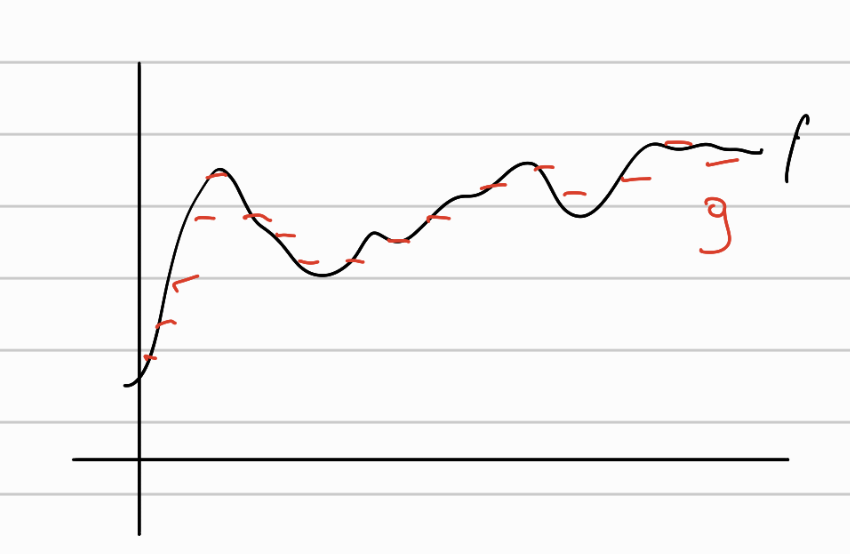
\includegraphics[width=0.7\linewidth]{img/screenshot002}
	\caption{I forgot to turn off page lines before exporting}
	\label{fig:screenshot002}
\end{figure}
In this case the function $g$ converges pointwise to $f$. The idea behind the \ito{} integral is that instead of pointwise convergence, we construct a step process that converges to our desired process in $L^{2}$. 
\begin{definition}
	Let $[S,T]\subset\R^{+}$ and $\seqttm{\F^{B}_{t}}$ be the natural filtration of a \bwm. We say that ${(f_{t})}_{t\in[S,T]}$ is a \emph{step process} if there exists
	\begin{equation*}
		S=t_{0}<\ldots<t_{n}=T
	\end{equation*}
	and a $\F^{B}_{t_{j}}$ adapted collection of random variables
	\begin{equation*}
		m_{0},\ldots,m_{n-1}\in L^{2}(\Pi,\dpr)
	\end{equation*}
	such that
	\begin{equation*}
		f_{t}=\sum_{j=0}^{n-1}m_{j}\indi_{[t_{j},t_{j+1}]}(t).
	\end{equation*}
\end{definition}
So the process is constant over deterministic points and the value must be given by some \rv{} adapted to \bwm: the \rv s are functions of \bwm{} trajectories up to a certain time.
We use 
\begin{equation*}
	M^{2}_{\mathsf{step}}[S,T]
\end{equation*}
to denote this class.
\begin{definition}
	\emph{\ito{} integral of a step process}. For every $f_{t}\in\mtus[S,t]$ we define the \ito{} integral of $f_{t}$ with respect to the \bwm{} by
	\begin{equation*}
		I(f):=:\int_{S}^{T}f_{t}\dbt:=\sum_{j=0}^{n-1}m_{j}(B_{t_{j+1}}-B_{t_{j}}).
	\end{equation*}
\end{definition}
This is analogous to the definition of Lebesgue integral for simple functions.
\begin{proposition}
	For every $f_{t}\in\mtus[S,T]$ we have
	\begin{equation*}
		I(f)\in L^{2}(\Omega,\dpr)
	\end{equation*}
	and
	\begin{equation*}
		\ev{\left(I(f)\right)^{2}}=\ev{\int_{S}^{T}f^{2}_{t}\dt}.
	\end{equation*}
	This result is called \emph{\ito{} isometry}.
\end{proposition}
We call it an isometry because
\begin{align*}
	\ev{(I(f))^{2}}&=\norm{I(f)}^{2}_{L^{2}(\Omega,\dif P)}\\
	&=\norm{f}^{2}_{L^{2}(\Omega\times[S,T],\dif P\times\dt)}
\end{align*}
where $\dif P$ is the Wiener measure and $\dt$ is the Lebesgue measure. The $L^{2}$ norm of the integral on the space is the same as the $L^{2}$ norm of the function on another space that is the product space $\Omega\times[S,T]$.
\begin{fancyproof}
	Define
	\begin{equation*}
		\Delta_{j}B:=B_{t_{j+1}}-B_{t_{j}}
	\end{equation*}
	and \begin{equation*}
		\Delta_{j}t:=t_{j+1}-t_{j}
	\end{equation*}
	with $\ev{\Delta_{j}B}=0$ and $\ev{\left(\Delta_{j}B\right)^{2}}=\Delta_{j}t$. We have that
	\begin{align*}
		I(f)^{2}&=\left[\sum_{j=0}^{n-1}m_{j}(B_{t_{j+1}}-B_{t_{j}})\right]^{2}\\
		&=\sum_{j=0}^{n-1}\sum_{k=1}^{n-1}m_{j}m_{k}\Delta_{j}B\Delta_{k}B\\
		&=\sum_{j=0}^{k-1}m^{2}_{j}\left(\Delta_{j}B\right)^{2}+2\sum_{k>j}^{max}m_{j}m_{k}\Delta_{j}B\Delta_{k}B.
	\end{align*}
	For $j=k$, using conditioning and tower property, we have
	\begin{align*}
		\ev{m_{j}m_{k}\Delta_{j}B\Delta_{k}B}&=\ev{m_{j}m_{k}\Delta_{j}B\ev{\Delta_{k}B|\F^{B}_{t_{j-1}}}}=0
	\end{align*}
	so we get
	\begin{align*}
		\ev{(I(f))^{2}}&=\sum_{j=0}^{n-1}\ev{m_{j}^{2}}\ev{\left(\Delta_{j}B\right)^{2}}\\
		&=\sum_{j=0}^{n-1}\ev{m_{j}^{2}}\Delta_{j}B<\infty
	\end{align*}
	because $m^{2}_{j}\in L^{2}(\Omega,\dpr)$ by construction. Now we need to prove the isometry. Take
	\begin{align*}
		f^{2}_{t}&=\sum_{j=0}^{n-1}\sum_{k=0}^{n-1}m_{j}m_{k}\indi_{[t_{j},t_{j+1}]}(t)\indi_{[t_{k},t_{k+1}]}(t)\\
		&=\sum_{j=0}^{n-1}\mu_{j}^{2}\indi_{t_{j},t_{j+1}}(t)
	\end{align*}
	so 
	\begin{equation*}
		\ev{\int_{S}^{T}f_{t}^{2}\dt}=\sum_{j=0}^{n-1}\ev{\left(m^{2}_{j}\right)}\Delta B_{t}.
	\end{equation*}
\end{fancyproof}
\begin{definition}
	We denote by $M^{2}[S,T]$ the class of random processes $f:\R^{+}\times\Omega\to\R$ such that
	\begin{enumerate}
		\item $(t,\omega)\mapsto f_{t}(\omega)$ is measurable for any $m\in[S,t]$ with respect to
		\begin{equation*}
			\left([S,m]\times\Omega,\B([S,m])\otimes\F^{B}_{m}\right)\to(\R,\B(\R));
		\end{equation*}
		\item it holds
		\begin{equation*}
			\ev{\int_{S}^{T}f^{2}\dt}<\infty.
		\end{equation*}
	\end{enumerate}
\end{definition} We have \emph{progressive measurability} if the mapping
\begin{equation*}
	(s,\omega)\mapsto X_{s}(\Omega)
\end{equation*}
is in \begin{equation*}
	\B([0,t])\otimes\F^{B}_{t}\qquad\every t\in[0,t].
\end{equation*}
\begin{proposition}
	Right continuous processes adapted to $B$ are progressively measurable.
\end{proposition}
So is \begin{equation*}
	\omega\mapsto\int_{0}^{t}X_{s}(\omega)\ds
\end{equation*}
$\F_{t}$-measurable? The answer is yes and we can check it by using the first part of the Fubini theorem. Progressive measurability ensures regularity on the time axis for the process. In general, we have that
\begin{equation*}
	\mtus[S,T]\underset{\text{dense}}{\subset}M^{2}[S,T].
\end{equation*}
\begin{lemma}
	If ${\left(f_{t}\right)}_{t\in[S,T]}\in\mtus[S,T]$ then there exists a sequence ${(\phi^{(n)})}_{n\in\N}\subset\mtus[S,T]$ such that
	\begin{equation*}
		\ev{\int_{S}^{T}\left|f(t)(\omega)-\phi^{(n)}_{t}(\omega)\right|^{2}}\dt\xrightarrow{n\to\infty}0.
	\end{equation*}
\end{lemma}
This means that we can always find a sequence of step processes that approximates $f$ in $L^{2}$. $\int_{S}^{T}\left|f(t)(\omega)-\phi^{(n)}_{t}(\omega)\right|^{2}\dt$ is nothing but the $L^{2}$ norm in $\Omega\times[S,T]$:
\begin{equation*}
	\norm{f_{\cdot}(\cdot)-\phi^{(n)}}^{2}_{L^{2}(\Omega\times[S,T],\dif P\times\dt)}
\end{equation*}
\begin{fancyproof}
	We just give the sketch of the proof. We will need the following cases:
	\begin{enumerate}[\circnum]
		\item $g_{t}\in M^{2}$ so $g_{t}$ is bounded and continuous: define
		\begin{equation*}
			\phi^{(n)}_{t}(\omega):=\sum_{j=0}^{n-1}g_{t_{j}}(\omega)\indi_{[t_{j},t_{j-1}]}(t)
		\end{equation*}
		so that $\phi_{t}^{n}\to g_{t}$.
		\item $g_{t}\in M^{2}$ only bounded: choose a sequence of smooth functions $\psi^{(n)}_{t}$ with compact support. We have
		\begin{equation*}
			\int_{0}^{t}\psi^{(n)}(t-s)\phi^{(n)}_{t}(s)\ds\to\int_{0}^{t}\psi(t-s)g_{s}\ds
		\end{equation*}
		and since $\psi^{(n)}(t)$ is smooth and of compact support then the limit is also continuous and bounded.
		\item $g_{t}\in M^{2}$ is neither bounded or continuous. Choose a transformation of $f$ that makes it bounded by applying step $2$.
	\end{enumerate}
\end{fancyproof}
So now that I have both my process $f_{t}\in M^{2}[S,T]$ and my sequence $\phi_{t}^{(n)}\subset\mtus[S,T]$ such that $\phi_{t}^{(n)}\xrightarrow{L^{2}}f_{t}$ we can now define the \ito{} integral for processes in $M^{2}[S,T]$.
\begin{definition}
	The \ito{} integral for a function $f_{t}\in M^{2}[S,T]$ is
	\begin{equation*}
	I(f_{t}):=	\int_{S}^{T}f_{t}\dif B_{t}:=L^{2}-\lim_{n}\int_{S}^{T}\phi^{(n)}_{t}\dbt.
	\end{equation*}
\end{definition}
Now we know that we can find such $\phi^{(n)}_{t}$ but does the limit exist? To ensure this, we need to check that ${(\phi^{(n)})}_{t}$ is a Cauchy sequence in $L^{2}$: then we know that the limit exists. So we must check that
\begin{equation*}
	\ev{\left(\int_{S}^{T}\phi^{(n)}_{t}\dbt-\int_{S}^{T}\phi^{(m)}_{t}\dbt\right)^{2}}\xrightarrow{n,m\to\infty}0
\end{equation*}
So
\begin{align*}
	\ev{\left(\int_{S}^{T}\phi^{(n)}_{t}\dbt-\int_{S}^{T}\phi^{(m)}_{t}\dbt\right)^{2}}&=\ev{\left(\int_{S}^{T}\left(\phi^{(n)}_{t}-\phi^{(m)}_{t}\right)\dbt\right)^{2}}\\
	\text{\footnotesize (\ito{} isometry)}\quad&=\ev{\int_{S}^{T}\left(\phi^{(n)}_{t}-\phi^{(m)}_{t}\right)^{2}\dt}\\
	&=\norm{\phi^{(n)}_{t}-\phi^{(m)}_{t}}_{L^{2}(\Omega\times[S,T])}\xrightarrow{n,m\to\infty}0
\end{align*}
and since this sequence converges it is also a Cauchy sequence. The key point is that we used \ito{} isometry to switch between $M^{2}$ and $L^{2}(\Omega\times[S,T])$. It is important to remember that even though we call this an ``integral'' we cannot use calculus rules, we cannot compute derivatives, we cannot apply any of the rules that apply to normal integrals.
\begin{theorem}
	\emph{\ito{} isometry for non-step processes}. Let ${(f_{t})}_{t\in[S,T]}\in M^{2}[S,T]$. Then
	\begin{equation*}
		\ev{\left(\int_{S}^{T}f_{s}\dbs\right)^{2}}=\ev{\int_{S}^{T}f_{s}^{2}\ds}.
	\end{equation*}
\end{theorem}
As before, we are switching between spaces:
\begin{equation*}
	\ubracketthin{\left(\int_{S}^{T}f_{s}\dbs\right)^{2}}_{\in L^{2}(\Omega\times[S,T])}\longmapsto\ubracketthin{\int_{S}^{T}f_{s}^{2}\ds}_{\in M^{2}}
\end{equation*}
(this is just an intuition, it's not formally correct).
\begin{fancyproof}
	We have
	\begin{equation*}
		\int_{S}^{T}f_{s}\dbs=L^{2}-\lim_{n}\int_{S}^{T}\phi_{s}^{(n)}\dbs
	\end{equation*}
	so
	\begin{align*}
	\ev{\left(\int_{S}^{T}f_{s}\dbs\right)^{2}}&=\lim_{n}\ev{\left(\int_{S}^{T}\phi_{s}^{(n)}\dbs\right)^{2}}\\
	\text{\footnotesize \ito{} isom.}\qquad&=\lim_{n}\ev{\int_{S}^{T}\left(\phi^{(n)}_{s}\right)^{2}\ds}\\
	&=\ev{\int_{S}^{T}f_{s}^{2}\ds}
	\end{align*}
	and this is true for the properties of $L^{2}$
 convergence because
 \begin{equation*}
 	\ev{\int_{S}^{T}f_{s}^{2}\ds}\in L^{2}(\Omega\times[S,T]).
 \end{equation*}
 \end{fancyproof}
What if we want to put the dependence on $\omega$? In other words, what is random in this stochastic integral? We may be tempted to write
\begin{equation*}
	I_{t}(\omega)=\int_{0}^{t}f_{s}(\omega)\dbs(\omega)
\end{equation*}
but this is wrong because it looks like we are fixing $\omega$ in the \bwm{} which would mean fixing the path. Truth is, we are in $L^{2}$ so we completely lose the dependence on the \textit{single} path, which gets ``averaged out'' in the integral that considers \textit{all} paths. We could write for the step processes
\begin{equation*}
	\int_{S}^{T}\phi^{(n)}_{s}(\omega)\dbs(\omega)
\end{equation*}
and this would be technically correct since we actually are fixing paths to check the single values, but for generic functions we should write something like
\begin{equation*}
	\left(\int_{0}^{t}f_{s}\dbs\right)(\omega)
\end{equation*}
but even this is a bit misleading. Taking the $L^{2}$ limit means taking all the possible trajectories so we are dealing with something more similar to a sequence:
\begin{equation*}
	{\left(\int_{S}^{T}f_{s}\dbs\right)}_{t\in[S,T]}.
\end{equation*}
Now we can look up to some properties:
\begin{itemize}
	\item \emph{``Linearity''}:
	\begin{equation*}
		\int_{S}^{t}f_{\omega}\dif B_{\omega}-\int_{S}^{s}f_{\omega}\dif B_{\omega}=\int_{s}^{t}f_{\omega}\dif B_{\omega}.
	\end{equation*}
	\item \emph{``Measurability''}:
	\begin{align*}
		I_{t}&=\int_{0}^{t}f_{s}\dbs\text{ is $\F^{B}_{t}$-measurable}
	\end{align*}
	and if $I_{t}^{(n)}\in\F^{B}_{t}$ then $I_{t}\in\F_{t}$.
	\item \emph{Martingale property}: this is the most important probabilistic argument why Riemann-Stieltjes integrals are not viable, since they would lose the martingale property.
	\begin{theorem}
		Let ${\left(f_{t}\right)}_{t\in[S,T]}\in M^{2}[S,T]$. The process ${\left(I_{t}\right)}_{t\in[S,T]}$ is a martingale with respect to $\F^{B}_{t}$.
	\end{theorem}
	\begin{fancyproof}
		\begin{enumerate}[\circnum]
			\item \textit{Adaptness}: it is verified. \hfill\faCheckCircle[regular]
			\item \textit{Integrability}: we have
			\begin{align*}
				\left(\ev{|I_{t}|}\right)^{2}&\leq\ev{I^{2}_{t}}\\
				&=\ev{\int_{S}^{T}f^{2}_{s}\ds}<\infty
			\end{align*}
			so it is verified.\hfill\faCheckCircle[regular]
			\item \textit{Martingale property}: we have that 
			\begin{equation*}
				I^{(n)}_{t}=\int_{0}^{t}\phi^{(n)}_{s}\dbs
			\end{equation*}
			so for $s>t$ we get
			\begin{align*}
				\ev{I^{(n)}_{t}|\F_{t}}&=\ev{\left.\int_{s}^{t}\phi^{(n)}_{t}\dif B_{r}+\int_{t}^{s}\phi^{(n)}_{t}\dif B_{r}\right|\F_{t}}\\
				&=\int_{s}^{t}\phi^{(n)}_{r}\dif B_{r}+\ev{\left.\int_{t}^{s}\phi^{(n)}_{r}\dif B_{r}\right|\F_{t}}
			\end{align*}
			so we need to prove that in the $L^{2}$ limit we have that 
			\begin{equation*}
				\ubracketthin{\int_{s}^{t}\phi^{(n)}_{r}\dif B_{r}}_{\to I^{(n)}_{t}}+\ubracketthin{\ev{\left.\int_{t}^{s}\phi^{(n)}_{r}\dif B_{r}\right|\F_{t}}}_{\to0}.
			\end{equation*}
			So we have
			\begin{align*}
				\ev{\left.\int_{t}^{s}\phi^{(n)}_{r}\dif B_{r}\right|\F_{t}}&=\ev{\left.\int_{t}^{s}\sum_{j=0}^{n-1}m_{j}^{(n)}\indi_{\left[t^{(n)}_{j},t^{(n)}_{j+1}\right]}(t)\dif B_{r}\right|\F_{t}}\\
				&=\sum_{t\leq t_{j}^{(n)}\leq t^{(n)}_{j+1}}\ev{\left.m^{(n)}_{j}\left(B_{t^{(n)}_{j+1}}-B_{t^{(n)}_{j}}\right)\right|\F_{t}}\\
				\text{\footnotesize tower p.ty}\quad&=\sum_{t\leq t^{(n)}_{j}\leq t^{(n)}_{j+1}}\evs\Biggl[m_{j}^{(n)}\ubracketthin{\ev{\left.B_{t_{j+1}}-B_{t_{j}}\right|\F_{t_{j}}}}_{=0}\Big|\F_{t}\Biggr]\\
				&=0
			\end{align*}
			so it is verified. \hfill\faCheckCircle[regular]
		\end{enumerate}
	\end{fancyproof}
	\item \emph{``Strict continuity''}: take the mapping
	\begin{equation*}
		t\mapsto\int_{s}^{t}f_{s}\dif B_{s}.
	\end{equation*}
	if $f_{s}\in\mtus[s,t]$ then
	\begin{equation*}
		\int_{s}^{t<T}f_{s}\dbs=\sum_{i=0}^{n-1}f_{i}\left(B_{t_{i+i}\wedge t}-B_{t_{i}\wedge t}\right)
	\end{equation*}
	so we have a linear composition of continuous functions, since step processes are continuous. But what if we want to extend to $M^{2}$?
	\begin{theorem}
		Let ${\left(f_{t}\right)}_{t\in[S,T]}\in M^{2}[S,T]$. Then ${(I_{t})}_{t\in[S,T]}$ has a continuous version
		\begin{equation*}
			{\left(\widetilde{I}_{t}\right)}_{t\in[S,T]}.
		\end{equation*}
	\end{theorem}
	So $\widetilde{I}_{t}(\omega)$ is continuous for almost every $\omega\in\R$ and
	\begin{equation*}
		\pr(I_{t}=\widetilde{I}_{t})=1\qquad\every S\leq t\leq T.
	\end{equation*}
	If $f_{t}\in M^{2}[S,T]$ then
	\begin{equation*}
		I_{t}=\int_{S}^{t}f_{s}\dbs
	\end{equation*}
	and
	\begin{align*}
		\ev{I_{t}}&=\ev{I_{s}}\\
		&=\int_{S}^{S}f_{s}\dbs=0
	\end{align*}
	which honestly makes sense.
\end{itemize}
We know that if $f_{t}\in M^{2}$ then there exists a function $f_{n}\in\mtus$ such that $f_{n}\xrightarrow{M^{2}}f$.
\begin{theorem}
	\emph{Continuous version}. Let ${(F_{t})}_{t\in[S,T]}\in M^{2}$. Then ${(I_{t})}_{t\in[S,T]}$ where $I_{t}=\int_{S}^{T}f_{s}\dbs$ has a continuous version $\widetilde{I}_{t}$.
\end{theorem}
This means that $\widetilde{I}_{t}$ is continuous and 
\begin{equation*}
	\pr(\widetilde{I}_{t}=I_{t})=1\qquad\every t\in[S,T].
\end{equation*}
\begin{fancyproof}
	Let $\phi^{(n)}_{t}\in \mtus:\phi_{t}\xrightarrow{M^{2}}f_{t}$. We know that \\
	\begin{equation*}
		I^{(n)}_{t}=\int_{0}^{t}\phi^{(n)}_{s}\dbs
	\end{equation*}
	is continuous. We also know that $I^{(n)}_{t}\xrightarrow{L^{2}}I_{t}$ by definition of \ito{} integral. We need to check that there exists $m_{k}$ such that $I^{(m_{k})}_{t}$ is uniformly Cauchy in the sense that 
	\begin{equation*}
		\sup_{S\leq t\leq T}\left|I^{(m_{k})}_{t}-I^{(m_{k+1})}_{t}\right|\xrightarrow{k\to\infty}0.
	\end{equation*}
	Uniform convergence preserves continuity so
	\begin{equation*}
		I^{(m_{k})}_{t}\to\widetilde{I}_{t}\quad\as{}
	\end{equation*}
	and $\widetilde{I}_{t}$ is continuous, but $I^{m}_{t}\xrightarrow{L^{2}}I_{t}$ so the theorem follows by uniqueness of limit.
	To check that the sequence is Cauchy we need to use Doob's martingale inequality:
	\begin{proposition}
		Let $(X_{t})$ be a martingale such that $t\mapsto X_{t}$ is almost surely continuous. Then $\every p\geq 1$, $t>0$,$\lambda>0$ we have
		\begin{equation*}
			\begin{carray}
				\pr\left(\sup_{0\leq t\leq T}|X_{t}|>\lambda\right)\leq\lambda^{-p}\ev{|X_{T}|^{p}}.
			\end{carray}
		\end{equation*}
	\end{proposition}
	So we get 
	\begin{align*}
		\pr\left(\sup_{S\leq t\leq T}\left|I^{(m)_{t}-I^{(n)}_{t}}\right|>\varepsilon\right)&\leq\frac{1}{\varepsilon^{3}}\ev{\left(I^{(m)}_{T}-I^{(n)}_{T}\right)^{2}}\\
		\text{\footnotesize \ito{} isom.}\qquad&\leq\frac{1}{\varepsilon^{2}}\evs\Bigg[\ubracketthin{\int_{S}^{T}\left|\phi^{(m)}_{s}-\phi^{(n)}_{s}\right|^{2}\ds}_{M^{2}}\Bigg]\xrightarrow{m,n\to\infty}0.
		\end{align*}
		Now we use this to check that there exists a suitable subsequence. Define
		\begin{equation*}
			A_{n}:=\left\{\omega\in\Omega:\sup_{S\leq t\leq T}\left|I^{(m_{k})}_{t}-I^{(m_{k+1})}_{t}\right|>2^{-k}\right\}.
		\end{equation*}
		choose $m_{k}$ such that 
		\begin{equation*}
			\pr(A_{k})\leq 2^{-k}.
		\end{equation*}
		In this way we have $\sum_{k}\pr(A_{k})<\infty$ and by Borel Cantelli this means that 
		\begin{equation*}
			\pr(\limsup A_{k})=0\implies\pr(\liminf A^{c}_{k})=1.
		\end{equation*}
		So we can call $\liminf A^{c}_{k}=\omega$ and say that 
		\begin{equation*}
			\exists\omega\in\Omega:\exists N(\omega)\;\every k>N(\omega),\sup_{S\leq t\leq T}\left|I^{m_{k}}_{t}(\omega)-I^{m_{k+1}}_{t}(\omega)\right|\leq 2^{-k}.
		\end{equation*}
Then let $k\to\infty$ and we have our result.		
\end{fancyproof}
\begin{remark}
	From now on we always consider the continuous version
	\begin{equation*}
		t\mapsto\int_{0}^{t}f_{s}\dbs\qquad\text{continuous a.s.}
	\end{equation*}
	And same goes for $\phi^{(n)}\to f$ with $\phi^{(n)}\subset\mtus$. We can improve this by removing the step condition and thus getting
	\begin{equation*}
		\int_{0}^{T}\phi^{(n)}_{m}\dbs\to\int_{s}^{t}f\dbs.
	\end{equation*}
\end{remark}
\begin{theorem}
	Take $X_{t}, Y_{t}\in\mtus$ and suppose 
	\begin{equation*}
		\pr\left(\left\{X_{t}=Y_{t}\;\every t\in[S,T]\right\}\right)=1.
	\end{equation*}
	Then
	\begin{equation*}
		\int_{S}^{T}X_{t}\dbt=\int_{S}^{T}Y_{t}\dbt\qquad\text{a.s.}
	\end{equation*}
\end{theorem}
\begin{theorem}
	Let $\tau$ be a stopping time with respect to $\F^{B}_{t}$, $\tau<t$. Then if $F\in M^{2}[0,T]$ also $f_{t}\indig{t:\tau}\in M^{2}[0,T]$ and
	\begin{equation*}
		I_{\tau}:=\int_{0}^{\tau}f_{s}\dbs\stackrel{\as{}}{=}\int_{0}^{T}f_{s}\indig{s<\tau}\dbs.
	\end{equation*}
\end{theorem}
This is the concept of stopping the integral $I_{t}$ at time $\tau$.
\chapter{Stochastic Calculus}
\section{Useless barrage of calculations}
\begin{lemma}
	Let $F\in M^{2}$ be a stochastic process in $[0,T]$ with
	\begin{equation*}
		[0,T]\times[0,T]\ni(u,v)\mapsto\ev{\left(f(u)-f(v)\right)^{2}}
	\end{equation*}
	continuous in $[0,T]\times[0,T]$. Let $\Pi_{n}$ be a partition of $[0,T]$
	\begin{equation*}
		\{0=t_{0}<t_{1}<\ldots<t_{n}=T\}
	\end{equation*}and define
	\begin{equation*}
		f^{\Pi_{n}}(t):=\sum_{j=1}^{n}f(t_{j-1})\indi_{[t_{j-1},t_{j}]}(t).
	\end{equation*}
	Then 
	\begin{equation*}
		f^{\Pi_{n}}\xrightarrow{M^{2}[0,T]}
	\end{equation*}
	as $|\Pi|\to0$.
\end{lemma}
\begin{fancyproof}
	We have
	\begin{align*}
		\ev{\int_{0}^{T}\left(f(t)-f^{\Pi_{n}}(t})\right)^{2}\dt&=\ev{\sum_{j}\int_{s_{j-1}}^{s_{j}}\left(f(t)-f(s_{j-1})\right)^{2}\dt}\\
		&=\sum_{j}\int_{{s}_{j-1}}^{s_{j}}\ev{f(t)-f(s_{j-1})^{2}\dt}\\
		&\leq\sum_{j}\int_{s_{j-1}}^{s_{j}}\sup_{\underset{\times(s_{j-1},s_{j})}{(u,v)\in(s_{j-1},s_{j})}}\ev{(f(u)-f(v))^{2}}\dt\\
		&\leq\sup_{\underset{\times(s_{j-1},s_{j})}{(u,v)\in(s_{j-1},s_{j})}}\ev{(f(u)-f(v))^{2}}\sum_{j=1}^{n}(s_{j}-s_{j-1})
	\end{align*}
	and this goes to 0 as $|\Pi_{n}|\to0$ by uniform continuity.
\end{fancyproof}
Take $X_{t}=B^{2}_{t}$. In normal calculus we would say
\begin{equation*}
	\dif X_{t}=2B_{t}\dbt\qquad B^{2}_{t}=\int_{0}^{T}2B_{s}\dbs
\end{equation*}
but this can't be true because
\begin{equation*}
	\ev{B^{2}_{t}}=t\neq\ev{\int_{0}^{T}2B_{s}\dbs}=0.
\end{equation*}
Now take a partition $\Pi_{n}$ of $[0,T]$, with $|\Pi_{n}|\to0$. This gives us
\begin{equation*}
	X_{t}^{(n)}=\sum_{t_{k}\in\Pi_{n}}B_{t_{n}}\indi_{[t_{n},t_{n+1}]}(t).
\end{equation*} 
This means that
\begin{align*}
	\int_{0}^{T}X_{t}^{(n)}\dbt&=:\sum_{t_{n}\in\Pi_{n}}B_{t_{n}}(B_{t_{n+1}}-B_{t_{n}})\\
	&\xrightarrow{L^{2}}\int_{0}^{T}B_{t'}\dif B_{t'}
\end{align*}
because $X^{(n)}_{t}\xrightarrow{M^{2}}B_{t}$. No now we have
\begin{align*}
	\int_{0}^{T}B_{t'}\dif B_{t'}&=\lim_{|\Pi_{n}|\to0}\sum_{t_{n}\in\Pi_{n}}B_{t_{n}}(B_{t_{n+1}}-B_{t_{n}})\\
	&=\unmezz\lim_{|\Pi_{n}|\to0}\sum_{t_{j}\in\Pi_{n}}\left[\left(B^{2}_{t_{n+1}}-B^{2}_{t_{n}}\right)-\left(B_{t_{n+1}}-B_{t_{n}}\right)^{2}\right]\\
	&=\unmezz\left(B^{2}_{t}-B^{2}_{0}\right)-\unmezz\ubracketthin{\lim_{|\Pi_{n}|\to0}\sum_{t_{n}\in\Pi_{n}}\left(B_{t_{n+1}}-B_{t_{n}}\right)^{2}}_{\claptext{quadratic var. in $L^{2}$ sense $\to t$}}\\
	&=\unmezz B^{2}_{t}-\unmezz t.
\end{align*}
So we proved that 
\begin{equation*}
	\int_{0}^{T}B_{t'}\dif B_{t'}=\unmezz B^{2}_{t}-\unmezz t
\end{equation*}
and this implies
\begin{equation*}
	\begin{carray}
		B_{t}^{2}=2\int_{0}^{t}B_{t'}\dif B_{t'}+t\\
		\Downarrow\\
		\dif B^{2}_{t}=2B_{t}\dbt+\dt
	\end{carray}
\end{equation*}
which is crazy because in normal analysis we would just toss $\dif B^{2}_{t}$ out of the windows being an infinitesimal of order 2 but here we are in the $L^{2}$ world and therefore it retains relevance. Now take
\begin{equation*}
	F^{(m)}(t)=\sum_{t_{n}\in\Pi_{n}}t_{n}\indi_{[t_{n},t_{n+1}]}(t).
\end{equation*}
We know that $F^{(m)}\xrightarrow{M^{2}}t$ so
\begin{equation*}
	\int_{0}^{t}s\dbs=\lim_{n}\ubracketthin{\sum_{t_{n}\in\Pi_{n}}t_{n}(B_{t_{n+1}}-B_{t_{n}})}_{\int_{0}^{T}f_{s}^{(n)}\dbs}
\end{equation*}
so we can write
\begin{align*}
	t_{B_{t}}&=\sum_{t_{n}\in\Pi_{n}}\left[t_{n+1}B_{t_{n+1}}-t_{n}B_{t_{n}}\right]\pm B_{t_{n}}t_{n+1}\\
	&=\sum_{t_{n}\in\Pi_{n}}\left[B_{t_{n}}(t_{n+1}-t_{n})+t_{n+1}(B_{t_{n+1}}-B_{t_{n}})\right]\pm t_{n}(B_{t_{n+1}}-B_{t_{n}})\\
	&=\ubracketthin{\sum_{t_{n}\in\Pi_{n}}B_{t_{n}}(t_{n+1}-t_{n})}_{\mathrm{I}}+\ubracketthin{\sum_{t_{n}\in\Pi_{n}}t_{n}(B_{t_{n+1}}-B_{t_{n}})}_{\mathrm{II}}-\ubracketthin{\sum_{t_{n}\in\Pi_{n}}(t_{n}-t_{n+1})\left(B_{t_{n+1}}-B_{t_{n}}\right)}_{\mathrm{III}}.
\end{align*}
Let's now study I, II and III separately.
\begin{itemize}
	\item $\mathrm{I}\xrightarrow[|\Pi_{n}|\to\infty]{\as{}}\int_{0}^{T}B_{s}\ds$ (for definition of Riemann);
	\item $\mathrm{II}\xrightarrow[|\Pi_{n}|\to\infty]{L^{2}}\int_{0}^{T}s\dbs$;
	\item $\mathrm{III}$: we have 
	\begin{align*}
		\mathrm{III}&=\left|\sum_{t_{n}\in \pi_{n}}\left(t_{n+1}-t_{n}\right)\left(B_{t_{n+1}}-B_{t_{n}}\right)\right|\\
		&\leq\max_{t_{n}\in\Pi_{n}}\left|B_{t_{n+1}}0B_{t_{n}}\right|\ubracketthin{\sum_{t_{n}\in\Pi_{n}}\left(t_{n+1}-t_{n}\right)}_{t}\xrightarrow[|\Pi_{n}|\to0]{\as{}}0.
	\end{align*}
\end{itemize}
So we get
\begin{align*}
	tB_{t}&=\mathrm{I}_{n}+\mathrm{II}_{n}+\mathrm{III}_{n}\\
	&\stackrel{\as{}}{=}\int_{0}^{T}B_{s}\ds+\int_{0}^{T}s\dbs+0.
\end{align*}
\section{Chain rule for \ito{} integral}
So, if we have 
\begin{equation*}
	X=h(B_{t})\qquad h:\R\to\R
\end{equation*}
and we want to compute the differential, if we apply the rules of classical calculus then we get $\dif X_{t}$ but it doesn't make sense: we need to apply \ito{} definition to get something similar to te chain rule for normal integrals.
\begin{definition}
	Let $t\geq 0$. A random process $\seqtm{X}$ adapted to $\F^{B}_{t}$ such that \\
	\begin{equation*}
		\int_{0}^{t}|X_{s}|\ds<\infty\;\as{}
	\end{equation*}
	is said to be \emph{$M^{1}[0,t]$}.
\end{definition}
\begin{definition}
	A random process is called an \emph{\ito{} process} if
	\begin{enumerate}
		\item $t\mapsto X_{t}$ is continuous a.s.;
		\item there exists a process 
		\begin{equation*}
			{(b_{s})}_{s\in[0,T]}\in M^{1}[0,T]
		\end{equation*}
		and
		\begin{equation*}
			{(\sigma_{s})}_{s\in[0,T]},\every t\geq0
		\end{equation*}
		such that
		\begin{equation*}
			X_{t}-X_{0}=\int_{0}^{t}b_{s}\ds+\int_{0}^{t}\sigma_{s}\ds\qquad\as{}
		\end{equation*}
	\end{enumerate}
\end{definition}
This is often written in concise notation: 
\begin{equation*}
	\dif X_{t}=b_{t}\dt+\sigma_{t}\dif B_{t}.
\end{equation*}
So \ito{} processes are the process enjoying the decomposition. So the increment is proportional to the time interval times a random quantity plus the increment of a \bwm{} scaled by the diffusion term.
\begin{theorem}
	Let $h:\R^{+}\times\R\to\R$ be $\mathcal{C}^{1}$ in the variable $t$ and $\mathcal{C}^{2}$ in the variable $x$. Define $X_{t}:=h(t,B_{t})$. Then $X_{t}$ is an \ito{} process and it is true that
	\begin{equation*}
		X_{t}-X_{0}=\int_{0}^{t}\left[\partial_{t}h(s,B_{s})+\unmezz\partial^{2}_{x} h(s,B_{s})\right]\ds+\int_{0}^{t}\partial_{x}h(s,B_{s})\dbs.
	\end{equation*} 
\end{theorem}
For example, if we set $h(x,t)=x^{2}$ which means $X_{t}=B^{2}_{t}$ we then have
\begin{equation*}
	\begin{larray}
		h(t,x)=x^{2}\\
		\partial_{x}h(t,x)=2x\\
		\partial^{2}_{x}h(t,x)=2
	\end{larray}
\end{equation*}
so using the fact that $X_{t}-X_{0}=\int_{0}^{t}\left[\partial_{t}h(s,B_{s})+\unmezz\partial^{2}_{x} h(s,B_{s})\right]\ds+\int_{0}^{t}\partial_{x}h(s,B_{s})\dbs$ we get
\begin{equation*}
	\ubracketthin{X_{t}-X_{0}}_{B^{2}_{t}-B^{2}_{0}}=\int_{0}^{t}\left(0+\unmezz\cdot2\right)\ds+2\int_{0}^{t}B_{s}\dbs.
\end{equation*}
Another special case is given when we have $h\in\mathcal{C}^{2}(\R)$ and $X_{t}=b(B_{t})$:
\begin{equation*}
	X_{t}-X_{0}=\int_{0}^{t}h'(B_{s})\dbs+\int_{0}^{t}h''(B_{s})\ds.
\end{equation*}
\begin{fancyproof}
	We prove the theorem assuming that the support $h$ is $[-k,k]$ for some $k>0$. Since the derivatives of $h$ are bounded we get
	\begin{equation*}
		\norm{h}+\norm{h'}+\norm{h''}\leq\infty.
	\end{equation*}
	Take $\Pi_{n}=\{0=t_{0}<t_{1},\ldots,t_{n}=T\}$. We have
	\begin{equation*}
		h(B_{t})-h(B_{0})=\sum_{i=1}^{n}\left(h(B_{t_{j}})-h(B_{t_{j-1}})\right)
	\end{equation*}
Now take the second order expression with Lagrange remainder:
\begin{align*}
	h(x)&=\sum_{k=0}^{n-1}\frac{h^{(x)}(a)}{k!}(x-a)^{k}+\frac{f^{(n)}(\xi)}{n!}(x-0)^{n}\\
	&=\sum_{j=1}^{n}\left[\cancel{h(B_{t_{j-1}})}+h'(B_{t_{j-1}})(B_{t_{j}}-B_{t_{j-1}})+\unmezz h''(\xi_{j})(B_{t_{j}}-B_{t_{j-1}})^{2}-\cancel{h(B_{t_{j-1}})}\right]\\
	&=\ubracketthin{\sum_{j=}^{n}h'(B_{t_{j-1}})(B_{t_{j}}-B_{t_{j-1}})}_{\mathrm{I}}+\ubracketthin{\unmezz\sum_{j=1}^{n}h''(\xi_{j})(B_{t_{j}}-B_{t_{j-1}})^{2}}_{\mathrm{II}}.
\end{align*}
So we need to show that 
\begin{enumerate}
	\item $\mathrm{I}\to\int_{0}^{t}h'(B_{s})\dbs$
	\item $\mathrm{II}\to\int_{0}^{t}h''(B_{s})\ds$
\end{enumerate}
as $|\Pi_{n}|\to0$.
\begin{enumerate}
	\item We write
	\begin{equation*}
		\sum_{j=1}^{h}h'(B_{t_{j-1}})(B_{t_{j}}-B_{t_{j-1}})=\int_{0}^{t}f_{s}^{\Pi_{n}}\dbs
	\end{equation*}
	with
	\begin{equation*}
		f^{\Pi_{n}}_{s}=\sum_{j=i}^{n}h'(B_{t_{j-1}})\indi_{(B_{t_{j-1}},B_{t_{j}})}\xrightarrow{M^{2}}h'B_{s}
	\end{equation*}
	since $\ev{\left(h'(B_{n})-h'(B_{n})\right)^{2}}$ is continuous on $[0,T]\times[0,T]$. We have
	\begin{equation*}
		\int_{0}^{t}f^{\Pi_{n}}\dbs\xrightarrow{L^{2}}\int_{0}^{t}h'(B_{s})\dbs
	\end{equation*}
	so we proved $\mathrm{I}$.
	\item We can write
	\begin{align*}
		\mathrm{II}&=\unmezz\sum_{j=1}^{n}h''(\xi_{j})\left(B_{t_{j}}-B_{t_{j-1}}\right)^{2}\\
		&=\unmezz\ubracketthin{\sum_{j=1}^{n}h''(B_{t_{j-1}})(B_{t_{j}}-B_{t_{j-1}})^{2}}_{\mathrm{II}_{a}}+\unmezz\ubracketthin{\sum_{j=1}^{n}\left(h''(\xi_{i})-h''(B_{t_{j-1}})\right)\left(B_{t_{j}}-B_{t_{j-1}}\right)^{2}}_{\mathrm{II}_{b}}.
	\end{align*}
	We must let $\mathrm{II}_{b}\to0$.
	\begin{align*}
		|\mathrm{II}_{b}|&\leq\sum_{j=1}^{n}\left|h''(\xi_{j})-h''(B_{t_{j-1}})\right|\left(B_{t_{j}}-B_{t_{j-1}}\right)^{2}\\
		&\leq\max_{j}\left\{\left|h''(\xi_{j})-h''(B_{t_{j-1}})\right|\sum_{i=1}^{n}\left(B_{t_{j}}-B_{t_{j-1}}\right)^{2}\right\}\\
		&\leq\ev{\max_{j}\left\{\left|h''(\xi_{j})-h''(B_{t_{j-1}})\right|\sum_{j=i}^{n}\left(B_{t_{j}}-B_{t_{j-1}}\right)^{2}\right\}}\\
		&\leq\ubracketthin{\sqrt{\ev{\max_{j}\left\{\left|h''(\xi_{j})-h''(B_{t_{j-1}})\right|^{2}\right\}}}\cdot}_{0}\ubracketthin{\sqrt{\ev{\left(\sum_{j=1}^{n}\left(B_{t_{j-1}}-B_{t_{j-1}}\right)^{2}\right)^{2}}}}_{t}.
	\end{align*}
	Since $s\to h''(B_{s})$ is uniformly continuous we have
	\begin{align*}
		\sum_{j=1}^{n}h''(B_{t_{j-1}})(B_{t_{j}}-B_{tj-1})^{2}&=\sum_{j=1}^{n}h''(B_{t_{j-1}})(t_{j}-t_{j-1})+\\
		&+\left[\sum_{i=1}^{n}h''(B_{t_{j-1}})\left((B_{t_{j}}-B_{t_{j-1}})^{2}(t_{j}-t_{j-1})\right)\right].
	\end{align*}
	Taking expectation of the second term yields
	\begin{align*}
		&\ev{\left[\sum_{j=1}^{n}h''(B_{t_{j-1}})\left(\left(B_{t_{j}}-B_{t_{j-1}}\right)^{2}-\Delta_{j}t\right)\right]^{2}}\\
		=&\ev{\sum_{j=1}^{n}\left|h''(B_{t_{j-1}})\right|^{2}\left[\left(B_{t_{j}}-B_{t_{j-1}}\right)^{2}-(t_{j}-t_{j-1})\right]^{2}}\\
		=&\ev{\left(h''(B_{t_{j-1}})\left(\Delta_{j}B^{2}-\Delta_{j}t\right)\right)\left(h''(B_{t_{k-1}})\left(\Delta_{k}B^{2}-\Delta_{k}t\right)\right)}\\
		=&\ev{\ev{\left(h''(B_{t_{j-1}})\left(\Delta_{j}B^{2}-\Delta_{j}t\right)\right)\left(h''(B_{t_{k-1}})\left(\Delta_{k}B^{2}-\Delta_{k}t\right)\right)}|\F_{t_{k-1}}}\\
		=&\ev{\Delta_{k}B^{2}-\Delta_{k}t|\F_{k-1}}\\
		=&0.
	\end{align*}
	So we have
	\begin{align*}
		&\ev{\sum_{j=1}^{n}\left|h^{(n)}\left(B_{t_{j-1}}\right)\right|^{2}\left[\left(B_{t_{j}}-B_{t_{j-1}}\right)^{2}-\left(t_{j}-t_{j-1}\right)\right]^{2}}\\
		\leq&\norm{h}\ev{\sum_{j=k}^{n}\left[\left(B_{t_{j}}-B_{t_{j-1}}\right)^{2}-\left(t_{j}-t_{j-1}\right)\right]^{2}}\\
		\leq&\norm{h}\sum_{j=1}^{n}\ev{\left[B^{2}_{t_{j}-t_{j-1}}-(t_{j}-t_{j-1})\right]^{2}}\\
		=&\norm{h}\sum_{j=1}^{n}(t_{j}-t_{j-1})^{2}\ubracketthin{\ev{(B^{2}_{t}-1)^{2}}}_{c}\\
		\leq&c\norm{h}|\Pi_{n}|\ubracketthin{\sum_{j=1}^{n}(t_{j}-t_{j-1})}_{t}\xrightarrow{|\Pi_{n}|\to0}0.
	\end{align*}
	In the last decomposition we still need to check that
	\begin{equation*}
		\sum_{j=1}^{n}h''(B_{t_{j-1}})(t_{j}-t_{j-1})\convas\int_{0}^{t}h''(B_{s})\ds.
	\end{equation*}
	By definition of Riemann integral the sum converges to $h''(B_{s})$. Under extra assumptions on $n$ we have
	\begin{equation*}
		X_{t}-X_{0}=\mathrm{I}_{a}+\mathrm{II}_{b}
	\end{equation*}
	and
	\begin{equation*}
		\mathrm{II}_{n}^{a}+\mathrm{II}_{n}^{b}+\mathrm{II}_{n}^{c}+\mathrm{II}_{n}^{d}=0
	\end{equation*}
	??
\end{enumerate}
\end{fancyproof}

This theorem had the extra assumption of $h$ having compact support. We now must get rid of this assumption. Take a general $h\in\mathcal{C}^{2}$. Fix $\varepsilon>0$ and let $\chi_{\varepsilon}$ be a cutoff function smooth such that
\begin{equation*}
	\indi_{B(0,\varepsilon)}\leq\chi_{\varepsilon}\leq\indi_{B(0,-\varepsilon)}.
\end{equation*}
\begin{figure}[H]
	\centering
	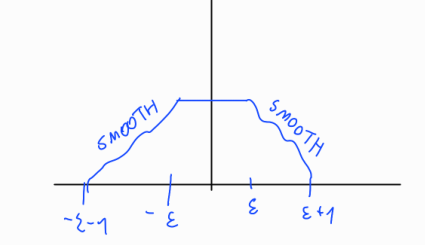
\includegraphics[width=0.5\linewidth]{img/screenshot003}
	\caption{Shape of the cutoff function.}
	\label{fig:screenshot003}
\end{figure}
Set $h_{\varepsilon}(x)=h(x)\chi_{\varepsilon}(x)$. This is smooth with compact support, which means that we can apply the previous theorem to $h_{\varepsilon}(x)$:
\begin{equation*}
	\begin{carray}
		h_{\varepsilon}(B_{t})-h_{\varepsilon}(B_{0})=\int_{0}^{t}h_{\varepsilon}'(B_{s})\dbs+\unmezz\int_{0}^{t}h''_{\varepsilon}(B_{s})\ds\\
		\text{and}\\
		\frac{\dif^{j}}{\dif x^{j}}h_{\varepsilon}(B_{s})=h^{(j)}(B_{s\wedge\tau(\varepsilon)})
	\end{carray}
\end{equation*}
where $\tau(\varepsilon)$ is the first exit time of the \bwm{} from $\varepsilon$:
\begin{equation*}
	\tau(\varepsilon)=\inf_{s}\left\{s>0:|B_{s}|\geq\varepsilon\right\}.
\end{equation*}
We know that 
\begin{align*}
	h\left(B_{t\wedge\tau(\varepsilon)}\right)-h\left(B_{0}\right)&=h_{\varepsilon}\left(B_{t\wedge\tau(\varepsilon)}\right)-h\left(B_{0}\right)\\
	&=\int_{0}^{t\wedge\tau(\varepsilon)}h'_{\varepsilon}(B_{s})\dbs+\int_{0}^{t\wedge\tau(\varepsilon)}h''_{\varepsilon}(B_{s})\ds\\
	&=\int_{0}^{T}h'_{\varepsilon}(B_{s})\indi_{[0,t\wedge\tau(\varepsilon)]}(t)\dbs+\unmezz\int_{0}^{T}h''_{\varepsilon}(B_{s})\indi_{[0,t\wedge\tau(\varepsilon)]}(s)\ds\\
	&=\int_{0}^{T}h(B_{s})\indi_{[0,t\wedge\tau(\varepsilon)]}(t)\dbs+\unmezz\int_{0}^{T}h'(B_{s})\indi_{[0,t\wedge\tau(\varepsilon)]}(s)\ds\\
	&=\int_{0}^{T}h'(B_{s})\indi_{[0,t\wedge\tau(\varepsilon)]}(s)\dbs+\unmezz\int_{0}^{T}h''(B_{s})\indi_{[0,t\wedge\tau(\varepsilon)]}(s)\ds\\
	&=\int_{0}^{t\wedge\tau(\varepsilon)}h'(B_{s})\dbs+\unmezz\int_{0}^{t\wedge\tau(\varepsilon)}h''(B_{s})\ds.
\end{align*}
We must remember that \bwm{} does not explode in finite time so as $\varepsilon\to\infty$ we have $\tau(\varepsilon)\to\infty$ so
\begin{equation*}
	h(B_{t})-h(B_{0})=\int_{0}^{t}h'(B_{s})\dbs+\unmezz\int_{0}^{t}\ds.
\end{equation*}
\begin{theorem}
	Let $\seqtm{X}$ be an \ito{} process with drift $b_{t}$ and diffusion $\sigma_{t}$. Let $h:\R^{+}\times\R\to\R$ be $\mathcal{C}^{1}$ in $t$ and $\mathcal{C}^{2}$ in $x$. Let $Y_{t}=h(t,X_{t})$. Then
	\begin{align*}
		Y_{t}-Y_{0}=&\int_{0}^{t}\left(\partial_{t}h(s,X_{s})+b_{s}\partial_{x}h(s,X_{s})+\unmezz\partial^{2}_{x}h(s,X_{s})\right)\ds+\int_{0}^{t}\sigma_{s}\partial_{x}h(s,X_{s})\dbs\\
		=&\int_{0}^{t}\left(\partial_{t}h(s,X_{s})+b_{s}\partial_{x}h(s,X_{s})+\unmezz\partial^{2}_{x}h(s,X_{s})\right)\ds+\\&+\int_{0}^{t}\partial_{x}h(s,X_{s})\ubracketthin{\left(b_{s}\ds+\sigma_{s}\dbs\right)}_{=\dif X_{s}}\\
		=&\int_{0}^{t}\partial_{x}h(s,X_{s})\dif X_{s}
	\end{align*}
	which is the integral with respect to an \ito{} process.
\end{theorem}
So here we have
\begin{equation*}
	\dif Y_{t}=\partial_{t}h(t,X_{t})\dt-\unmezz\partial^{2}_{x}h(t,Y_{t})\dt+\partial_{x}h(x,X_{t})\dif X_{t}.
\end{equation*}
Remember, this is just shorthand notation. Why we needed shorthand notation for \textit{this}, it honestly eludes me.
\section{Formal rules of \ito{} calculus and solving a SDE}
We have seen that
\begin{equation*}
	\begin{rarray}
		(\dt)^{2}=0\\
		\left(\dbt\right)^{2}=\dt\\
		\dbt\dt=\dt\dbt=0
	\end{rarray}
\end{equation*}
and the general formula of the integral for an \ito{} process is
\begin{equation*}
	\dif X_{t}=b_{t}\dt+\sigma_{t}\dbt.
\end{equation*}
With $Y_{t}=h(t,X_{t})$ we have the expansion
\begin{equation*}
	h(t,x)=h(t_{0},x_{0})+\partial_{t}h(t_{0},x_{0})(t-t_{0})+\partial_{x}h(t_{0},x_{0})\ldots
\end{equation*}
So we get 
\begin{align*}
	\ubracketthin{Y_{t+\dt}-Y_{t}}_{\dif Y_{t}}=&\partial_{t}h(t,X_{t})\dt+\partial_{x}h(t,Y_{t})\dif X_{t}+\unmezz\partial^{2}_{t}h(t,X_{t})\left(\dt\right)^{2}+\partial^{2}_{t,x}h(t,x)\dt\dbt+\\&+\unmezz\partial^{2}_{x}h(t,X_{t})\left(\dbt\right)^{2}\\
	=&\partial_{t}h(t,X_{t})\dt+\partial_{x}h(t,X_{t})\left(b_{t}\dt+\sigma_{t}\dbt\right)+\ubracketthin{\partial^{2}_{t,x}h(t,X_{t})\dt\left(b_{t}\dt+\sigma_{t}\dbt\right)}_{=0}+\\
	&+\unmezz\partial^{2}_{x}h(t,X_{t})\left(b_{t}\dt+\sigma_{t}\dbt\right)\\
	=&\left(\partial_{t}h(t,X_{t})+b_{t}\partial_{x}h(t,X_{t})\right)\dt+\sigma_{t}\partial_{x}h(t,B_{t})+\unmezz\partial^{2}_{x}h(t,X_{t})\left(b^{2}_{t}(\dt)^{2}+\sigma^{2}_{t}(\dbt)^{2}\right)+\\
	&+2b\sigma_{t}\dt\dbt\\
	=&\left(\dt h(t,X_{t})+b_{t}\partial_{x}h(t,X_{t})\dt+\sigma_{t}\partial_{x}h(t,X_{t})\dbt\right)+\unmezz\partial^{2}_{x}h(t,X_{t})\sigma^{2}_{t}\dt.
\end{align*}
So now, going back to our SDE
\begin{equation*}
	X_{t+\dt}-X_{t}=\ubracketthin{h(t,X_{t})\dt}_{\claptext{deterministic}}+\sigma(t,X_{s})\dbt
\end{equation*}
we have the tools to give meaning to this ``normal'' Cauchy problem:
\begin{equation*}
	\begin{cases}
		X_{t}-X_{0}=\ubracketthin{\int_{0}^{t}b(s,X_{s})\ds}_{\claptext{normal Riemann}}+\ubracketthin{\int_{0}^{t}\sigma(s,X_{s})\dbs}_{\claptext{\ito}}\\
		X_{0}=x\in\R.
	\end{cases}
\end{equation*}
Given $b$ and $\sigma$, is there a process $X_{t}$ that solves this problem? Remember that the solution we are looking for is a process ${(X_{t})}_{t\in[0,T]}$. Now we must prove uniqueness and existence of this process.
\begin{theorem}
	Let $t>0$ and suppose that there exist some constants $C,D>0$ such that for every $t\in[0,T]$ it is true that
	\begin{enumerate}
		\item 
		\begin{equation*}
			\left|b(t,x)-b(t,y)\right|+\left|\sigma(t,x)-\sigma(t,y)\right|\leq D|x-y|;
		\end{equation*}
		\item 
		\begin{equation*}
			\left|b(t,x)\right|+\left|\sigma(t,x)\right|\leq C(1+|x|)
		\end{equation*}
	\end{enumerate}
	for any $x,y\in\R$. Then there exists a continuous process
	\begin{equation*}
		{\left(X^{x}_{t}\right)}_{t\in[0,T]}
	\end{equation*}
	on the Wiener space sch that $X^{x}_{t}$ is a solution of the SDE and
	\begin{enumerate}
		\item $\ev{\int_{0}^{t}\left|X^{x}_{s}\right|^{2}\ds}<\infty$;
		\item $X^{x}_{t}$ is a.s. continuous;
		\item $X^{x}_{t}$ is adapted to ${\left(\F^{B}_{t}\right)}_{t\in[0,T]}$.
	\end{enumerate}
	Such process is unique: let $Y^{x}_{t}$ be another solution of the SDE. Then
	\begin{equation*}
		\pr\left(X^{x}_{t}=Y^{x}_{t}\;\every t\in[0,T]\right)=1.
	\end{equation*}
\end{theorem}
\end{document} 


%THIS IS THE DARK AGE OF LOVE   $\cdot$